\documentclass[12pt, titlepage]{article}

\usepackage{fullpage}
\usepackage[round]{natbib}
\usepackage{multirow}
\usepackage{booktabs}
\usepackage{tabularx}
\usepackage{graphicx}
\usepackage{float}
\usepackage{hyperref}
\hypersetup{
    colorlinks,
    citecolor=blue,
    filecolor=black,
    linkcolor=red,
    urlcolor=blue
}

\input{../../Comments}
\input{../../Common}

\newcounter{acnum}
\newcommand{\actheacnum}{AC\theacnum}
\newcommand{\acref}[1]{AC\ref{#1}}

\newcounter{ucnum}
\newcommand{\uctheucnum}{UC\theucnum}
\newcommand{\uref}[1]{UC\ref{#1}}

\newcounter{mnum}
\newcommand{\mthemnum}{M\themnum}
\newcommand{\mref}[1]{M\ref{#1}}

\begin{document}

\title{Module Guide for \progname{}} 
\author{\authname}
\date{\today}

\maketitle

\pagenumbering{roman}

\section{Revision History}

\begin{tabularx}{\textwidth}{p{3cm}p{2cm}X}
\toprule {\bf Date} & {\bf Version} & {\bf Notes}\\
\midrule
Date 1 & 1.0 & Notes\\
Date 2 & 1.1 & Notes\\
\bottomrule
\end{tabularx}

\newpage

\section{Reference Material}

This section records information for easy reference.

\subsection{Abbreviations and Acronyms}

\renewcommand{\arraystretch}{1.2}
\begin{tabular}{l l} 
  \toprule		
  \textbf{symbol} & \textbf{description}\\
  \midrule 
  AC & Anticipated Change\\
  DAG & Directed Acyclic Graph \\
  M & Module \\
  MG & Module Guide \\
  OS & Operating System \\
  R & Requirement\\
  SC & Scientific Computing \\
  SRS & Software Requirements Specification\\
  \progname & Explanation of program name\\
  UC & Unlikely Change \\
  \wss{etc.} & \wss{...}\\
  \bottomrule
\end{tabular}\\

\newpage

\tableofcontents

\listoftables

\listoffigures

\newpage

\pagenumbering{arabic}

\section{Introduction}

Decomposing a system into modules is a commonly accepted approach to developing
software.  A module is a work assignment for a programmer or programming
team~\citep{ParnasEtAl1984}.  We advocate a decomposition
based on the principle of information hiding~\citep{Parnas1972a}.  This
principle supports design for change, because the ``secrets'' that each module
hides represent likely future changes.  Design for change is valuable in SC,
where modifications are frequent, especially during initial development as the
solution space is explored.  

Our design follows the rules layed out by \citet{ParnasEtAl1984}, as follows:
\begin{itemize}
\item System details that are likely to change independently should be the
  secrets of separate modules.
\item Each data structure is implemented in only one module.
\item Any other program that requires information stored in a module's data
  structures must obtain it by calling access programs belonging to that module.
\end{itemize}

After completing the first stage of the design, the Software Requirements
Specification (SRS), the Module Guide (MG) is developed~\citep{ParnasEtAl1984}. The MG
specifies the modular structure of the system and is intended to allow both
designers and maintainers to easily identify the parts of the software.  The
potential readers of this document are as follows:

\begin{itemize}
\item New project members: This document can be a guide for a new project member
  to easily understand the overall structure and quickly find the
  relevant modules they are searching for.
\item Maintainers: The hierarchical structure of the module guide improves the
  maintainers' understanding when they need to make changes to the system. It is
  important for a maintainer to update the relevant sections of the document
  after changes have been made.
\item Designers: Once the module guide has been written, it can be used to
  check for consistency, feasibility, and flexibility. Designers can verify the
  system in various ways, such as consistency among modules, feasibility of the
  decomposition, and flexibility of the design.
\end{itemize}

The rest of the document is organized as follows. Section
\ref{SecChange} lists the anticipated and unlikely changes of the software
requirements. Section \ref{SecMH} summarizes the module decomposition that
was constructed according to the likely changes. Section \ref{SecConnection}
specifies the connections between the software requirements and the
modules. Section \ref{SecMD} gives a detailed description of the
modules. Section \ref{SecTM} includes two traceability matrices. One checks
the completeness of the design against the requirements provided in the SRS. The
other shows the relation between anticipated changes and the modules. Section
\ref{SecUse} describes the use relation between modules.

\section{Anticipated and Unlikely Changes} \label{SecChange}

This section lists possible changes to the system. According to the likeliness
of the change, the possible changes are classified into two
categories. Anticipated changes are listed in Section \ref{SecAchange}, and
unlikely changes are listed in Section \ref{SecUchange}.

\subsection{Anticipated Changes} \label{SecAchange}

Anticipated changes are the source of the information that is to be hidden
inside the modules. Ideally, changing one of the anticipated changes will only
require changing the one module that hides the associated decision. The approach
adapted here is called design for
change.

\begin{description}
\item[\refstepcounter{acnum} \actheacnum \label{acHardware}:] The specific
  hardware on which the software is running.
\item[\refstepcounter{acnum} \actheacnum \label{acInput}:] The format of the
  initial input data.
\item ...
\end{description}

\wss{Anticipated changes relate to changes that would be made in requirements,
design or implementation choices.  They are not related to changes that are made
at run-time, like the values of parameters.}

\subsection{Unlikely Changes} \label{SecUchange}

The module design should be as general as possible. However, a general system is
more complex. Sometimes this complexity is not necessary. Fixing some design
decisions at the system architecture stage can simplify the software design. If
these decision should later need to be changed, then many parts of the design
will potentially need to be modified. Hence, it is not intended that these
decisions will be changed.

\begin{description}
\item[\refstepcounter{ucnum} \uctheucnum \label{ucIO}:] Input/Output devices
  (Input: File and/or Keyboard, Output: File, Memory, and/or Screen).
\item ...
\end{description}

\section{Module Hierarchy} \label{SecMH}

This section provides an overview of the module design. Modules are summarized
in a hierarchy decomposed by secrets in Table \ref{TblMH}. The modules listed
below, which are leaves in the hierarchy tree, are the modules that will
actually be implemented.

\begin{description}
\item [\refstepcounter{mnum} \mthemnum \label{mHH}:] Hardware-Hiding Module
\item ...
\end{description}


\begin{table}[h!]
\centering
\begin{tabular}{p{0.3\textwidth} p{0.6\textwidth}}
\toprule
\textbf{Level 1} & \textbf{Level 2}\\
\midrule

{Hardware-Hiding Module} & ~ \\
\midrule

\multirow{7}{0.3\textwidth}{Behaviour-Hiding Module} & ?\\
& ?\\
& ?\\
& ?\\
& ?\\
& ?\\
& ?\\ 
& ?\\
\midrule

\multirow{3}{0.3\textwidth}{Software Decision Module} & {?}\\
& ?\\
& ?\\
\bottomrule

\end{tabular}
\caption{Module Hierarchy}
\label{TblMH}
\end{table}

\section{Connection Between Requirements and Design} \label{SecConnection}

The design of the system is intended to satisfy the requirements developed in the SRS. In this stage, the system is decomposed into modules. The connection between requirements and modules is listed in Table~\ref{TblRT}.

\subsection*{Design Decisions}

\begin{description}
	\item[\textbf{Security}] To satisfy security and privacy requirements (FR21--FR23, SR-IR1, SR-PR1--2), the system implements end-to-end encryption for data at rest and in transit using industry-standard encryption protocols. User authentication employs session-based tokens with automatic timeout after 60 minutes of inactivity.
	\item[\textbf{Real-time Performance}] To meet the requirement for real-time feedback (FR13--14, PR-SL1--2), the computer vision processing pipeline is optimized to provide analysis results within 1~second of detecting form deviations. This is achieved through efficient pose estimation algorithms and selective processing of critical joint angles.
	\item[\textbf{Offline Capability}] To address reliability requirements (PR-RFT2, MS-AD1), the system implements local caching of exercise instructions and video queuing for uploads. This ensures users can access exercise information and record sessions even without internet connectivity, with automatic synchronization when connection is restored.
	\item[\textbf{Modular Exercise Library}] To support extensibility (PR-CR1, PR-SER1), the exercise library is designed as a modular system where new exercises and joint types can be added without modifying core analysis logic. Each exercise type has its own parameter set defining acceptable ranges and form criteria.
	\item[\textbf{Two-Camera View Analysis}] To address the risk of 3D motion measurement with 2D cameras, the system supports analysis from the sagittal view as primary, with optional frontal view for enhanced accuracy. The analysis algorithms are designed to work with single or multiple camera angles.
\end{description}

\section{Module Decomposition} \label{SecMD}

Modules are decomposed according to the principle of ``information hiding.'' The \emph{Secrets} field in a module decomposition is a brief statement of the design decision hidden by the module. The \emph{Services} field specifies \emph{what} the module will do without documenting \emph{how} to do it. If the entry is \emph{OS}, this means that the module is provided by the operating system or by standard programming language libraries. \emph{\progname{}} means the module will be implemented by the \progname{} software. Only the leaf modules in the hierarchy have to be implemented.

\subsection{Hardware Hiding Modules (M1)}

\begin{description}
	\item[Secrets:] The data structure and algorithm used to implement the virtual hardware.
	\item[Services:] Serves as a virtual hardware used by the rest of the system. This module provides the interface between the hardware and the software, including camera access, screen display, audio output, and device sensors. The system can use it to capture video, display outputs, or accept touch inputs.
	\item[Implemented By:] Android~OS
\end{description}

\subsection{Behaviour-Hiding Module}

\begin{description}
	\item[Secrets:] The contents of the required behaviours.
	\item[Services:] Includes programs that provide externally visible behaviour of the system as specified in the software requirements specification (SRS) documents. This module serves as a communication layer between the hardware-hiding module and the software decision module. The programs in this module will need to change if there are changes in the SRS.
	\item[Implemented By:] --
\end{description}

\subsubsection{Authentication Module (M2)}
\begin{description}
	\item[Secrets:] The implementation details of user authentication, session management, and credential verification.
	\item[Services:] Handles user login, logout, session creation, and session timeout. Verifies user credentials against stored records and manages authentication tokens. Enforces 60-minute inactivity timeout as per SR-AR3.
	\item[Implemented By:] \progname{}
	\item[Type of Module:] Abstract Object
	\item[Related Requirements:] FR1, FR1.1, SR-AR1, SR-AR3
\end{description}

\subsubsection{User Account Management Module (M3)}
\begin{description}
	\item[Secrets:] The structure and validation logic for user account data, including patient and physiotherapist profiles.
	\item[Services:] Creates and manages user accounts for both patients and physiotherapists. Validates registration data including government ID, license numbers (for PTs), and invite codes (for patients). Stores and retrieves user profile information securely.
	\item[Implemented By:] \progname{}
	\item[Type of Module:] Abstract Data Type
	\item[Related Requirements:] FR1.1, FR1.2, FR1.3, FR2
\end{description}

\subsubsection{Organization Linking Module (M4)}
\begin{description}
	\item[Secrets:] The algorithm for generating, validating, and managing access codes that link patients to physiotherapists.
	\item[Services:] Generates unique access codes for physiotherapists to share with patients. Validates patient-submitted access codes and establishes the patient--PT relationship. Manages the patient list for each physiotherapist. Handles patient account deletion requests from PTs.
	\item[Implemented By:] \progname{}
	\item[Type of Module:] Abstract Object
	\item[Related Requirements:] FR1.3, FR2, FR3, FR18
\end{description}

\subsubsection{Exercise Library Module (M5)}
\begin{description}
	\item[Secrets:] The storage structure and retrieval methods for exercise information, including instructions, media, and form parameters.
	\item[Services:] Maintains a library of at least ten knee exercises with detailed instructions, demonstration media, and form parameters. Provides exercise information to users on demand. Supports caching for offline access.
	\item[Implemented By:] \progname{}
	\item[Type of Module:] Abstract Data Type
	\item[Related Requirements:] FR5, MS-AD1
\end{description}

\subsubsection{Exercise Program Management Module (M6)}
\begin{description}
	\item[Secrets:] The data structures and business logic for managing patient-specific exercise programs, including customization and progress tracking.
	\item[Services:] Allows physiotherapists to create and customize exercise programs for individual patients, including sets, reps, rest times, and weekly limits. Tracks patient exercise completion and progress over time. Enforces PT-defined limitations on exercise frequency and intensity.
	\item[Implemented By:] \progname{}
	\item[Type of Module:] Abstract Object
	\item[Related Requirements:] FR6, FR10, FR11, FR22, FR27
\end{description}

\subsubsection{Video Capture Module (M7)}
\begin{description}
	\item[Secrets:] The implementation of video recording, including camera configuration, frame rate management, and recording controls.
	\item[Services:] Captures video of users performing exercises at minimum 720p resolution and 30~fps. Performs pre-capture environment checks (lighting, framing). Provides recording controls (start, stop, retry). Ensures video meets minimum quality standards before proceeding to analysis.
	\item[Implemented By:] \progname{}
	\item[Type of Module:] Abstract Object
	\item[Related Requirements:] FR7, FR15, FR26, UHR-EOU3
\end{description}

\subsubsection{Video Storage Module (M8)}
\begin{description}
	\item[Secrets:] The mechanism for storing, retrieving, and managing video files, including local caching and cloud synchronization.
	\item[Services:] Stores recorded exercise videos securely (encrypted at rest per SR-IR1). Manages local storage and cloud upload queuing. Handles upload retry logic when network is unavailable. Retrieves stored videos for patient and PT review. Implements automatic backup functionality.
	\item[Implemented By:] \progname{}
	\item[Type of Module:] Abstract Object
	\item[Related Requirements:] FR21, SR-IR1, PR-RFT2, MS-MNT1
\end{description}

\subsubsection{Feedback Generation Module (M11)}
\begin{description}
	\item[Secrets:] The rules and logic for converting analysis results into user-friendly feedback messages and instructions.
	\item[Services:] Generates real-time corrective feedback messages based on form analysis results. Provides step-by-step exercise guidance. Creates descriptive messages for form deviations specifying required adjustments. Triggers safety warnings for dangerous movements.
	\item[Implemented By:] \progname{}
	\item[Type of Module:] Library
	\item[Related Requirements:] FR13, FR14, FR16, PR-SCR1
\end{description}

\subsubsection{Reporting Module (M12)}
\begin{description}
	\item[Secrets:] The format and generation logic for exercise session reports and progress summaries.
	\item[Services:] Generates comprehensive session reports including completion rate, form score, pain level, and patient feedback. Creates progress summaries showing improvement over time. Generates alerts for repeated incorrect attempts or concerning patterns. Formats reports for PT review.
	\item[Implemented By:] \progname{}
	\item[Type of Module:] Library
	\item[Related Requirements:] FR17, FR19, FR20, FR25
\end{description}

\subsubsection{Dashboard Module (M13)}
\begin{description}
	\item[Secrets:] The user interface layout and interaction logic for patient and physiotherapist dashboards.
	\item[Services:] Displays patient exercise history, progress charts, and upcoming exercises. Shows PT patient list with status indicators and alerts. Provides access to video review and report viewing. Enables PT comments on patient sessions. Presents analytics and visualizations of exercise data.
	\item[Implemented By:] \progname{}
	\item[Type of Module:] Abstract Object
	\item[Related Requirements:] FR18, FR19, FR24, FR25
\end{description}

\subsection{Software Decision Module}

\begin{description}
	\item[Secrets:] The design decision based on mathematical theorems, physical facts, or programming considerations. The secrets of this module are not described in the SRS.
	\item[Services:] Includes data structure and algorithms used in the system that do not provide direct interaction with the user.
	\item[Implemented By:] --
\end{description}

\subsubsection{Computer Vision Processing Module (M9)}
\begin{description}
	\item[Secrets:] The specific computer vision algorithms and implementation details for pose detection, joint tracking, and body landmark identification.
	\item[Services:] Processes video frames to detect and track body landmarks using pose estimation. Identifies key joints relevant to knee exercises (hip, knee, ankle, foot). Extracts coordinate data for joint positions across video frames. Handles varying lighting conditions and camera angles. Implements the core CV library integration (e.g., OpenCV, MediaPipe).
	\item[Implemented By:] \progname{}
	\item[Type of Module:] Abstract Data Type
	\item[Related Requirements:] FR8, FR12
\end{description}

\subsubsection{Form Analysis Module (M10)}
\begin{description}
	\item[Secrets:] The mathematical models and algorithms for calculating joint angles, range of motion, and determining form correctness based on exercise parameters.
	\item[Services:] Calculates joint angles from landmark coordinates with $\pm5^{\circ}$ accuracy. Measures range of motion with $\pm10\%$ accuracy. Compares measured values against exercise-specific acceptable ranges. Detects form deviations and classifies severity. Identifies dangerous movements requiring immediate halt. Measures time-under-tension and exercise duration.
	\item[Implemented By:] \progname{}
	\item[Type of Module:] Library
	\item[Related Requirements:] FR12, FR13, FR14, PR-PAR1, PR-PAR2, PR-SCR1
\end{description}

\subsubsection{Data Encryption Module (M14)}
\begin{description}
	\item[Secrets:] The encryption algorithms, key management, and cryptographic protocols used to secure patient data.
	\item[Services:] Encrypts patient data at rest and in transit using industry-standard protocols. Manages encryption keys securely. Provides methods for encrypting and decrypting data as needed by other modules. Ensures compliance with healthcare data security requirements.
	\item[Implemented By:] \progname{}
	\item[Type of Module:] Library
	\item[Related Requirements:] FR21, SR-IR1
\end{description}

\subsubsection{Access Control Module (M15)}
\begin{description}
	\item[Secrets:] The authorization logic and permission management system that enforces data access policies.
	\item[Services:] Enforces role-based access control for patients and physiotherapists. Ensures patients can only access their own data. Ensures PTs can only access data for patients in their patient list. Logs unauthorized access attempts. Validates user permissions before allowing data operations.
	\item[Implemented By:] \progname{}
	\item[Type of Module:] Abstract Object
	\item[Related Requirements:] FR23, SR-PR1, SR-PR2
\end{description}


\section{Traceability Matrix} \label{SecTM}

This section shows two traceability matrices: between the modules and the
requirements and between the modules and the anticipated changes.

% the table should use mref, the requirements should be named, use something
% like fref
\begin{table}[H]
\centering
\begin{tabular}{p{0.2\textwidth} p{0.6\textwidth}}
\toprule
\textbf{Req.} & \textbf{Modules}\\
\midrule
R1 & \mref{mHH}, \mref{mInput}, \mref{mParams}, \mref{mControl}\\
R2 & \mref{mInput}, \mref{mParams}\\
R3 & \mref{mVerify}\\
R4 & \mref{mOutput}, \mref{mControl}\\
R5 & \mref{mOutput}, \mref{mODEs}, \mref{mControl}, \mref{mSeqDS}, \mref{mSolver}, \mref{mPlot}\\
R6 & \mref{mOutput}, \mref{mODEs}, \mref{mControl}, \mref{mSeqDS}, \mref{mSolver}, \mref{mPlot}\\
R7 & \mref{mOutput}, \mref{mEnergy}, \mref{mControl}, \mref{mSeqDS}, \mref{mPlot}\\
R8 & \mref{mOutput}, \mref{mEnergy}, \mref{mControl}, \mref{mSeqDS}, \mref{mPlot}\\
R9 & \mref{mVerifyOut}\\
R10 & \mref{mOutput}, \mref{mODEs}, \mref{mControl}\\
R11 & \mref{mOutput}, \mref{mODEs}, \mref{mEnergy}, \mref{mControl}\\
\bottomrule
\end{tabular}
\caption{Trace Between Requirements and Modules}
\label{TblRT}
\end{table}

\begin{table}[H]
\centering
\begin{tabular}{p{0.2\textwidth} p{0.6\textwidth}}
\toprule
\textbf{AC} & \textbf{Modules}\\
\midrule
\acref{acHardware} & \mref{mHH}\\
\acref{acInput} & \mref{mInput}\\
\acref{acParams} & \mref{mParams}\\
\acref{acVerify} & \mref{mVerify}\\
\acref{acOutput} & \mref{mOutput}\\
\acref{acVerifyOut} & \mref{mVerifyOut}\\
\acref{acODEs} & \mref{mODEs}\\
\acref{acEnergy} & \mref{mEnergy}\\
\acref{acControl} & \mref{mControl}\\
\acref{acSeqDS} & \mref{mSeqDS}\\
\acref{acSolver} & \mref{mSolver}\\
\acref{acPlot} & \mref{mPlot}\\
\bottomrule
\end{tabular}
\caption{Trace Between Anticipated Changes and Modules}
\label{TblACT}
\end{table}

\section{Use Hierarchy Between Modules} \label{SecUse}

In this section, the uses hierarchy between modules is
provided. \citet{Parnas1978} said of two programs A and B that A {\em uses} B if
correct execution of B may be necessary for A to complete the task described in
its specification. That is, A {\em uses} B if there exist situations in which
the correct functioning of A depends upon the availability of a correct
implementation of B.  Figure \ref{FigUH} illustrates the use relation between
the modules. It can be seen that the graph is a directed acyclic graph
(DAG). Each level of the hierarchy offers a testable and usable subset of the
system, and modules in the higher level of the hierarchy are essentially simpler
because they use modules from the lower levels.

\wss{The uses relation is not a data flow diagram.  In the code there will often
be an import statement in module A when it directly uses module B.  Module B
provides the services that module A needs.  The code for module A needs to be
able to see these services (hence the import statement).  Since the uses
relation is transitive, there is a use relation without an import, but the
arrows in the diagram typically correspond to the presence of import statement.}

\wss{If module A uses module B, the arrow is directed from A to B.}

\begin{figure}[H]
\centering
%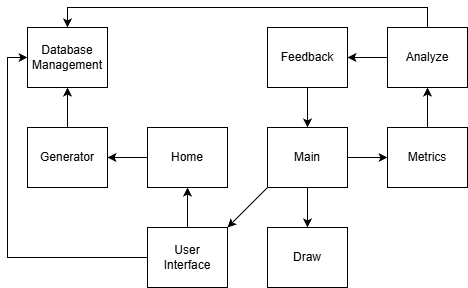
\includegraphics[width=0.7\textwidth]{UsesHierarchy.png}
\caption{Use hierarchy among modules}
\label{FigUH}
\end{figure}

%\section*{References}

\section{User Interfaces}

\wss{Design of user interface for software and hardware.  Attach an appendix if
needed. Drawings, Sketches, Figma}

\section{Design of Communication Protocols}

\wss{If appropriate}

\section{Timeline}

\wss{Schedule of tasks and who is responsible}

\wss{You can point to GitHub if this information is included there}

\bibliographystyle {plainnat}
\bibliography{../../../refs/References}

\newpage{}

\end{document}